
\documentclass[tikz]{standalone}

\usepackage{tikz}


%\pagestyle{empty}

\begin{document}



\tikzset{every picture/.style={line width=0.75pt}} %set default line width to 0.75pt        

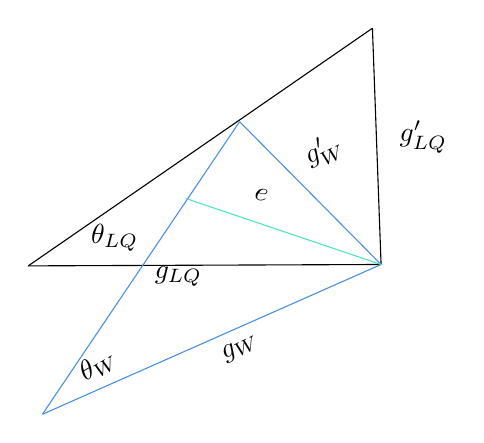
\begin{tikzpicture}[x=0.75pt,y=0.75pt,yscale=-1,xscale=1]
%uncomment if require: \path (0,300); %set diagram left start at 0, and has height of 300

%Straight Lines [id:da1512744683535726] 
\draw    (439.5,55) -- (273.67,169.5) ;


%Straight Lines [id:da5289128073072314] 
\draw    (439.5,55) -- (443.67,168.83) ;


%Straight Lines [id:da2226150120378121] 
\draw    (273.67,169.5) -- (443.67,168.83) ;


%Straight Lines [id:da3656294825730808] 
\draw [color={rgb, 255:red, 74; green, 144; blue, 226 }  ,draw opacity=1 ]   (375.5,100) -- (443.67,168.83) ;


%Straight Lines [id:da020018035136474266] 
\draw [color={rgb, 255:red, 74; green, 144; blue, 226 }  ,draw opacity=1 ]   (375.5,100) -- (280.5,241) ;


%Straight Lines [id:da2223254386394361] 
\draw [color={rgb, 255:red, 74; green, 144; blue, 226 }  ,draw opacity=1 ]   (280.5,241) -- (443.67,168.83) ;


%Straight Lines [id:da5867109106022379] 
\draw [color={rgb, 255:red, 80; green, 227; blue, 194 }  ,draw opacity=1 ]   (349.5,137) -- (443.67,168.83) ;



% Text Node
\draw (315.33,156) node   {$\theta _{LQ}$};
% Text Node
\draw (307.33,217.33) node [rotate=-330.09]  {$\theta _{W}$};
% Text Node
\draw (346,174.67) node   {$g_{LQ}$};
% Text Node
\draw (376,209.33) node [rotate=-334.41]  {$g_{W}$};
% Text Node
\draw (464,107.33) node   {$g'_{LQ}$};
% Text Node
\draw (416,114) node [rotate=-334.41]  {$g'_{W}$};
% Text Node
\draw (386,135.33) node [rotate=-18.03]  {$e$};


\end{tikzpicture}

\end{document}